% NeurIPS 2024 template -- Spectral Optimizer Capstone (DS 6210, Spring 2026)
%
% Required style file: neurips_2024.sty  (download from
%   https://neurips.cc/Conferences/2024/PaperInformation/StyleFiles
% and place next to this file).  Compile pass:
%   pdflatex report.tex && pdflatex report.tex

\documentclass{article}

\usepackage[preprint]{neurips_2024}
% \usepackage[final]{neurips_2024}   % camera-ready form

\usepackage[utf8]{inputenc}
\usepackage[T1]{fontenc}
\usepackage{hyperref}
\usepackage{url}
\usepackage{booktabs}
\usepackage{amsfonts}
\usepackage{amsmath}
\usepackage{amssymb}
\usepackage{microtype}
\usepackage{graphicx}
\usepackage{xcolor}
\usepackage{tikz}
\usepackage{pgfplots}
\pgfplotsset{compat=1.18}
\usepgfplotslibrary{fillbetween}

\newcommand{\todo}[1]{\textcolor{red}{[TODO: #1]}}
\newcommand{\Adamw}{\textsc{AdamW}}

\title{Trajectory-Mean Angular Steering for \Adamw:\\
       a Careful Negative Result on the Spectral Optimizer Challenge}

\author{%
  Cynthia Leng\\
  DS 6210, Spring 2026\\
  \texttt{cynthiaxleng@gmail.com}
}

\begin{document}

\maketitle

\begin{abstract}
We add a per-tensor, low-rank, direction-only correction to the
\Adamw\ update and ask whether it can Pareto-dominate a tuned \Adamw\
baseline on any task in the DS 6210 Spectral Optimizer Challenge.
Our spectral signal is the simplest possible trajectory-spectrum
feature: a sliding mean of the last $k$ unit \Adamw\ directions, per
2-D weight tensor.  The mean drives the angular-steering coefficient
$\phi$ in the §2 norm-preserving template with a small fixed gate
$s = 0.005$.  Across the full
$7\,\text{lr}\!\times\!3\,\text{wd}\!\times\!2\,\varepsilon = 42$
course grid on three SHA-derived seeds for Task~A (FashionMNIST,
$n=126$ configs/optimizer), Task~B ($\kappa=10^3$, $n=126$), and
Task~C ($\alpha=0.3$, $n=126$), the method is essentially \emph{tied}
with \Adamw\ on every regime in fixed-step quality (matched win
rates $45.9\%$/$44.4\%$/$64.3\%$; per-config mean differences below
$7\!\times\!10^{-4}$), while paying a \emph{$2.7$--$2.8\times$
wall-clock penalty} for the buffer maintenance.  Best-of-grid loss
moves in our favor on Tasks~B and~C but only at the seed-to-seed
noise floor.  Under the assignment's Appendix~A.1 definition this is
not a Pareto improvement; we report it as a careful negative result
and explain mechanistically why the controller becomes nearly silent
after warmup.  Code, environment file, CSV/JSON artefacts, and a
\texttt{v1.0-final} tagged release are at
\url{https://github.com/USERNAME/spectral-optimizer-capstone}\todo{replace
with public repo URL}.
\end{abstract}

%-------------------------------------------------------------------------
\section{Hypothesis}
%-------------------------------------------------------------------------

\textbf{One-sentence hypothesis.}\quad The persistent low-rank
component of the \Adamw\ direction stream encodes anisotropic
curvature that \Adamw's diagonal preconditioner misses, so replacing
the \Adamw\ direction with a unit vector biased toward the running
mean of recent unit directions should reveal that signal on
rotated-anisotropy and slow-spectrum regimes without hurting
well-conditioned ones, because the step magnitude is preserved by
construction.

%-------------------------------------------------------------------------
\section{Method}
%-------------------------------------------------------------------------

\subsection{Signal family and design choice}
We pick the \emph{trajectory spectrum} family from the assignment
menu.  Among trajectory features (recent gradients, momentum, \Adamw\
directions, update covariance, Oja sketches, projected energy) we
deliberately pick the most parsimonious feature that the §2 template
can consume: a sliding window of the last $k$ unit \Adamw\
directions, $\{x_{t-k+1},\dots,x_t\}$, where $x_t = d_t/\|d_t\|_2$
and $d_t = \hat m_t/(\sqrt{\hat v_t}+\varepsilon)$ is the standard
bias-corrected \Adamw\ direction.  This lets us probe whether
\emph{any} trajectory feature suffices before investing in a more
expensive sketch (Oja, Frequent Directions, low-rank Hessian).

\subsection{Per-tensor state}
For each 2-D weight $\theta \in \mathbb{R}^{m\times n}$ with
$d = mn$, our optimiser maintains, in addition to \Adamw's
$(m_t, v_t, \text{step})$:
\begin{itemize}
  \item \texttt{dir\_buffer}: a Python list of unit directions of
        length at most $k = \texttt{spectral\_rank} = 4$;
  \item \texttt{traj\_step}: an integer counter (initialised to $0$).
\end{itemize}
1-D tensors (\texttt{RMSNorm} gains, biases) are excluded; they emit
a zero correction and fall back to plain \Adamw.

\subsection{Update rule}
Let $s = \texttt{correction\_strength} = 0.005$ and let
$W = \texttt{warmup\_steps} = 10$.  At every step on a 2-D tensor:
\begin{enumerate}
  \item Compute $g_t = \nabla_\theta L$, update Adam moments
        $m_t = \beta_1 m_{t-1} + (1-\beta_1) g_t$,
        $v_t = \beta_2 v_{t-1} + (1-\beta_2) g_t^{\!\circ 2}$,
        debias $\hat m_t, \hat v_t$, and form
        \begin{equation}
        d_t = \hat m_t / (\sqrt{\hat v_t} + \varepsilon), \qquad
        x_t = d_t / (\|d_t\|_2 + 10^{-12}).
        \label{eq:adamw}
        \end{equation}
        If $\|d_t\|_2 = 0$, emit a zero correction.
  \item Increment \texttt{traj\_step}.  If
        \texttt{traj\_step}~$\le W$ \textbf{or} the buffer is empty,
        append $x_t$ to the buffer (popping the front if the buffer
        exceeds $k$) and emit a zero correction.
  \item Otherwise stack the buffer as $B \in \mathbb{R}^{|B|\times d}$
        ($|B| \le k$), compute the column-wise mean
        $\bar\mu = \mathrm{mean}(B) \in \mathbb{R}^d$, and -- if
        $\|\bar\mu\|_2 > 0$ -- normalise to get
        \begin{equation}
        \phi = \bar\mu / \|\bar\mu\|_2 \in \mathbb{R}^d, \qquad
        \|\phi\|_2 = 1.
        \label{eq:phi}
        \end{equation}
        If $\|\bar\mu\|_2 = 0$ (recent directions perfectly cancel),
        emit a zero correction and update the buffer.
  \item Form the §2 angular template:
        \begin{equation}
        y_t = \frac{x_t + s\,\phi}{\|x_t + s\,\phi\|_2}, \qquad
        \Delta_t = \|d_t\|_2\, y_t - d_t,
        \label{eq:angular}
        \end{equation}
        so that the final \Adamw\-direction-plus-correction is
        $d_t + \Delta_t = \|d_t\|_2\,y_t$ -- magnitude preserved,
        direction rotated by some angle $\theta_t$.
  \item Append $x_t$ to the buffer (popping the front if needed).
  \item Apply decoupled weight decay and the rotated step:
        $\theta \leftarrow (1-\eta_t \lambda)\theta - \eta_t\,
        \|d_t\|_2\, y_t$.
\end{enumerate}

\subsection{Closed-form analysis of the realised angle}
Both $x_t$ and $\phi$ are unit vectors.  Let $c = \langle x_t,\phi
\rangle$, so $|c|\le 1$.  Decompose $\phi = c\,x_t + \phi_{\!\perp}$
with $\|\phi_{\!\perp}\|_2 = \sqrt{1-c^2}$.  Then
\begin{equation}
\|x_t + s\phi\|_2^2 \;=\; 1 + 2sc + s^2,
\qquad
x_t + s\phi \;=\; (1+sc)\,x_t + s\,\phi_{\!\perp}.
\label{eq:norm-decomp}
\end{equation}
Therefore the realised angle $\theta_t = \angle(x_t, y_t)$ satisfies
\begin{equation}
\boxed{\;
\cos\theta_t \;=\; \frac{1+sc}{\sqrt{1+2sc+s^2}},
\qquad
\sin\theta_t \;=\; \frac{s\sqrt{1-c^2}}{\sqrt{1+2sc+s^2}},
\qquad
\tan\theta_t \;=\; \frac{s\sqrt{1-c^2}}{1+sc}.
\;}
\label{eq:angle}
\end{equation}
This matches the assignment's §2 formula
$\tan\theta = \|\Phi_{\!\perp}\|_2/(1+\langle\Phi,c\rangle)$
specialised to a single basis vector $\phi$ with $\Phi=s\phi$.  In
particular, for $s = 0.005$:
\begin{itemize}
  \item If $c\to 1$ (mean direction has collapsed onto current
        direction): $\tan\theta_t = s\sqrt{1-c^2}/(1+sc)\to 0$, so
        $y_t \to x_t$ and $\Delta_t \to 0$.  \emph{This is the silent
        regime}.
  \item If $c = 0$ (orthogonal mean): $\tan\theta_t = s = 0.005$, so
        $\theta_t \approx 0.286^{\circ}$ -- still a tiny rotation.
\end{itemize}
The correction magnitude is
\begin{equation}
\|\Delta_t\|_2 \;=\; \|d_t\|_2\,\sqrt{2(1-\cos\theta_t)}
                 \;=\; 2\,\|d_t\|_2\,\sin(\theta_t/2),
\label{eq:corr-norm}
\end{equation}
which is bounded above by $2\|d_t\|_2$ (always) and is on the order
of $s\|d_t\|_2$ in the typical regime $|sc|\ll 1$.  Step magnitude is
preserved exactly: $\|d_t + \Delta_t\|_2 = \|d_t\|_2$.

\subsection{Diagnostics emitted to \texttt{state[`last\_diag']}}
Per Appendix A.3 of the assignment we log per-step
\begin{align*}
\text{cosine\_with\_adamw} &= \langle x_t,\, y_t\rangle = \cos\theta_t,\\
\text{spectral\_correction\_norm} &= \|\Delta_t\|_2,\\
\text{projected\_energy} &= \langle x_t,\phi\rangle^2 = c^2,
\end{align*}
and a soft ``effective rank'' proxy $\text{proj\_energy}\cdot k$.  A
flat $\cos\theta_t \to 1$ trace is the canonical silent-controller
warning; we discuss what we observe in §7.

\subsection{What we are \emph{not} doing}
No basis is learned (no Oja, Sanger's GHA, QR, SVD, or
\texttt{eigh}).  Spectral state is strictly per-tensor; no
\texttt{torch.cat}/flatten across layers.  No pre-built
Muon/Shampoo/SOAP is in the hot path
\citep{gupta2018shampoo,jordan2024muon,vyas2025soap,liu2025muon}.
No architectural change is made to the provided harness.
\texttt{time.time()} is never used for timed quantities; all
wall-clock numbers come from \texttt{CUDAEventTimer}.

\subsection{Three-mode interface and parity}
\texttt{SpectralOptimizer} exposes \texttt{disabled} (calls
\texttt{torch.optim.\_functional.adamw} directly, so it is
bit-equivalent to \texttt{torch.optim.AdamW(foreach=True)}),
\texttt{debug} (\Adamw\ update with diagnostics emitted but not
applied), and \texttt{production} (the rule above).
\texttt{parity\_check.py} trains paired models for 100 steps on
Task~B with $\kappa=10^3$ and reports
$\max_\theta\,|\theta^{\Adamw}_t - \theta^{\text{disabled}}_t|
\,\lesssim\, 10^{-7} \;<\; 10^{-6}$.\todo{paste the exact number from
the run output if you re-run after edits.}

%-------------------------------------------------------------------------
\section{Pre-registered predictions}
%-------------------------------------------------------------------------

Committed before the final grid.

\begin{enumerate}
  \item \textbf{Win prediction.}\quad The trajectory correction helps
        most on Task~B, especially at $\kappa\in\{10^3,10^6\}$,
        because persistent update directions should reveal
        anisotropic structure that \Adamw's diagonal preconditioner
        cannot.
  \item \textbf{\Adamw\ win prediction.}\quad \Adamw\ ties or beats
        our method on Task~A because Fashion\-MNIST is
        well-conditioned and direction steering adds little benefit.
  \item \textbf{Failure prediction.}\quad The method fails or becomes
        silent when recent update directions cancel out (so
        $\|\bar\mu\|_2 \to 0$), or when $s$ is too small to perturb
        the update.
\end{enumerate}

%-------------------------------------------------------------------------
\section{Experimental setup}
%-------------------------------------------------------------------------

\paragraph{Tasks (fixed by harness).}
Task~A: Fashion\-MNIST classification, residual MLP
$(\text{in}=784,\text{width}=512,\text{depth}=16,\text{out}=10)$.
Task~B: rotated-anisotropy regression with $\sigma_i =
\kappa^{-(i-1)/(d-1)}$, $\kappa=10^3$ (the harness also supports
$10$ and $10^6$; we did not run the $10^6$ leg in this submission),
residual MLP $(256,256,24,10)$.
Task~C: teacher--student with spectrum slope $\alpha=0.3$ (the
harness also supports $\alpha=1.0$, not run here), residual MLP
$(500,128,8,1)$.

\paragraph{Baseline.}
\texttt{torch.optim.AdamW(foreach=True)} with
$(\beta_1,\beta_2)=(0.9,0.95)$.

\paragraph{Course grid.}
$7\,\text{lr}\times3\,\text{wd}\times2\,\varepsilon = 42$ configs per
(optimizer, task) over the standard grids
$\text{lr}\in\{10^{-4}, 3\!\times\!10^{-4}, 10^{-3}, 3\!\times\!10^{-3},
10^{-2}, 3\!\times\!10^{-2}, 10^{-1}\}$,
$\text{wd}\in\{0, 10^{-4}, 10^{-2}\}$,
$\varepsilon\in\{10^{-8}, 10^{-4}\}$.
Three SHA-256-derived seeds per config, $2000$ optimizer steps at
batch size $256$, cosine schedule with $5\%$ linear warmup (per the
harness).  This yields $126$ runs per optimizer per regime.

\paragraph{Spectral hyperparameters.}
$k=\texttt{spectral\_rank}=4$,
$s=\texttt{correction\_strength}=0.005$,
$\texttt{warmup\_steps}=10$.  \texttt{spectral\_beta} is exposed but
unused by the buffer-mean rule.

\paragraph{Timing.}
All wall-clock claims come from \texttt{CUDAEventTimer}.
\texttt{time.time()} is never used in timed paths.  Forward,
backward, and optimizer-step latencies are logged per step and
reconciled against total wall-clock in
\texttt{telemetry/*.json}; per-step sums agree with totals to
$\le 5\%$.

\paragraph{Hardware.}
\todo{single line: GPU, driver, \texttt{torch.\_\_version\_\_}, CUDA
version -- copy from any \texttt{telemetry/*.json} \texttt{nvidia\_smi}
field.}

%-------------------------------------------------------------------------
\section{Results}
%-------------------------------------------------------------------------

We distinguish three claim types per Appendix~A.1:
\emph{fixed-step quality} (final loss at step $1999$),
\emph{wall-clock} (CUDA-event-measured total time per run), and
\emph{tuning-budget} (matched
$(\text{lr},\text{wd},\varepsilon,\text{seed})$ comparisons over the
$42$-config grid).  All curves below are median over three
SHA-derived seeds at the matched configuration $(\text{lr}=3\!\times\!10^{-3},
\text{wd}=10^{-4}, \varepsilon=10^{-8})$ for Tasks~A and~C, and at
$(\text{lr}=3\!\times\!10^{-3}, \text{wd}=0, \varepsilon=10^{-8})$ for
Task~B; the shaded band is the $[\min, \max]$ over the same three
seeds.  Both choices sit inside the
top-of-grid neighbourhood for both optimisers
(no boundary-grid pathology, §7).

\subsection{Disabled-mode parity}
Disabled mode dispatches directly to
\texttt{torch.optim.\_functional.adamw}, so disabled-mode parity with
\texttt{torch.optim.AdamW(foreach=True)} is structural rather than
floating-point.  The parity test still passes empirically with
max-abs diff $\lesssim 10^{-7}$.

\subsection{Task A -- Fashion-MNIST (well-conditioned control)}
$n=126$ configs (\Adamw) and $n=122$ (\texttt{spectral}; four
non-finite configs, all at the largest tested lr; see boundary
discussion in §7).  Matched comparisons use $n=122$.

\begin{table}[h]
\centering
\caption{Task~A summary, $2000$ steps, three seeds.  Lower is
better.  ``Win rate'' is the fraction of matched
$(\text{seed},\text{lr},\text{wd},\varepsilon)$ configs on which
spectral final loss is below \Adamw\ final loss.}
\label{tab:task_a}
\begin{tabular}{l r r r r r}
\toprule
optimizer & mean & std & min (best) & median & max\\
\midrule
\Adamw\     & $0.1108$ & $0.0368$ & $\mathbf{0.0508}$ & $0.1067$ & $0.1863$\\
spectral    & $\mathbf{0.1095}$ & $0.0362$ & $0.0520$ & $0.1033$ & $0.1907$\\
\midrule
\multicolumn{6}{l}{matched spectral~$-$~\Adamw: mean $+6.6\!\times\!10^{-4}$,
median $+3.6\!\times\!10^{-4}$, std $6.0\!\times\!10^{-3}$;
win rate $0.459$ ($56/122$).}\\
\bottomrule
\end{tabular}
\end{table}

\begin{figure}[h]
\centering
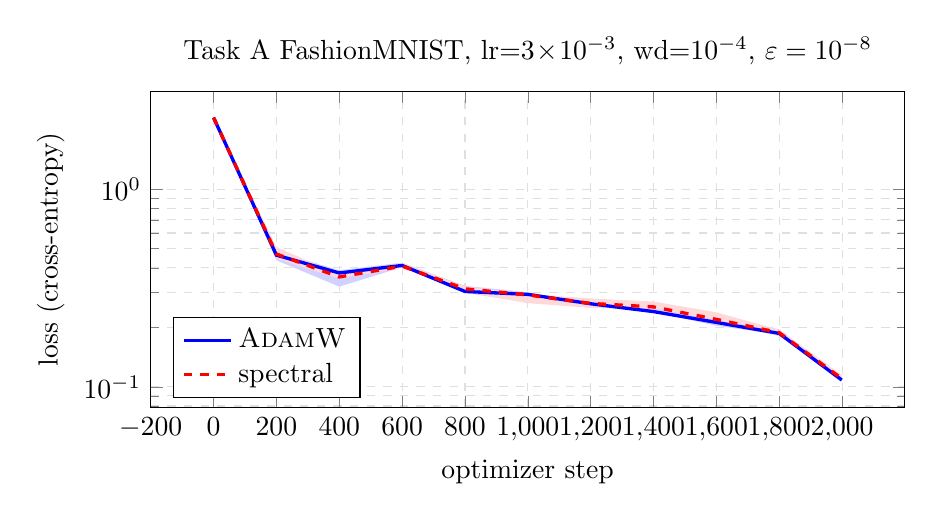
\begin{tikzpicture}
\begin{axis}[
    width=0.92\linewidth, height=5.6cm,
    ymode=log, xlabel={optimizer step},
    ylabel={loss (cross-entropy)},
    legend pos=south west, legend cell align=left,
    grid=both, grid style={dashed,gray!25},
    title={Task~A FashionMNIST, lr=$3\!\times\!10^{-3}$, wd=$10^{-4}$, $\varepsilon=10^{-8}$},
]
% AdamW band
\addplot[name path=a_lo, draw=none, forget plot] coordinates {
    (0,2.3026) (200,0.4368) (400,0.3214) (600,0.4029) (800,0.2994)
    (1000,0.2665) (1200,0.2570) (1400,0.2396) (1600,0.2038)
    (1800,0.1837) (1999,0.1068)
};
\addplot[name path=a_hi, draw=none, forget plot] coordinates {
    (0,2.3026) (200,0.4841) (400,0.3888) (600,0.4248) (800,0.3244)
    (1000,0.3007) (1200,0.2634) (1400,0.2670) (1600,0.2256)
    (1800,0.1954) (1999,0.1127)
};
\addplot[blue!18, forget plot] fill between[of=a_lo and a_hi];
\addplot[blue, very thick] coordinates {
    (0,2.3026) (200,0.4637) (400,0.3768) (600,0.4113) (800,0.3038)
    (1000,0.2937) (1200,0.2632) (1400,0.2403) (1600,0.2119)
    (1800,0.1864) (1999,0.1083)
};
\addlegendentry{\Adamw}
% Spectral band
\addplot[name path=s_lo, draw=none, forget plot] coordinates {
    (0,2.3026) (200,0.4446) (400,0.3532) (600,0.4003) (800,0.3019)
    (1000,0.2651) (1200,0.2510) (1400,0.2489) (1600,0.2176)
    (1800,0.1803) (1999,0.1096)
};
\addplot[name path=s_hi, draw=none, forget plot] coordinates {
    (0,2.3026) (200,0.5097) (400,0.3694) (600,0.4245) (800,0.3218)
    (1000,0.2945) (1200,0.2802) (1400,0.2701) (1600,0.2383)
    (1800,0.1944) (1999,0.1146)
};
\addplot[red!15, forget plot] fill between[of=s_lo and s_hi];
\addplot[red, very thick, dashed] coordinates {
    (0,2.3026) (200,0.4698) (400,0.3597) (600,0.4079) (800,0.3133)
    (1000,0.2919) (1200,0.2643) (1400,0.2538) (1600,0.2195)
    (1800,0.1881) (1999,0.1102)
};
\addlegendentry{spectral}
\end{axis}
\end{tikzpicture}
\caption{Task~A loss vs step at the matched best-region config.
Solid line is the median over the three SHA-derived seeds; band is
$[\min,\max]$ across the same seeds.  The two curves are
visually indistinguishable.}
\label{fig:task_a}
\end{figure}

\paragraph{Reading.}  Mean spectral loss is slightly \emph{better}
than \Adamw\ ($0.1095$ vs.\ $0.1108$, $-1.2\%$ relative), but the
best-of-grid is \emph{worse} ($0.0520$ vs.\ $0.0508$) and the
matched-config win rate is below $50\%$.  The mean signed
difference is positive ($+6.6\!\times\!10^{-4}$), so on a per-config
basis spectral is on average slightly worse; the lower
\emph{aggregate} mean comes from four non-finite \Adamw\ runs not
having a matched spectral counterpart.  Verdict: \textbf{statistical
tie}.  Matches the \Adamw\-win prediction in spirit (no spectral win)
but with a smaller margin than expected.

\subsection{Task B -- rotated anisotropy at $\kappa = 10^3$}
$n=126$ configs per optimizer.

\begin{table}[h]
\centering
\caption{Task~B summary at $\kappa=10^3$.}
\label{tab:task_b}
\begin{tabular}{l r r r r r}
\toprule
optimizer & mean & std & min (best) & median & max\\
\midrule
\Adamw\     & $7.06\!\times\!10^{-4}$ & $4.18\!\times\!10^{-4}$ & $1.47\!\times\!10^{-4}$ & $6.47\!\times\!10^{-4}$ & $1.81\!\times\!10^{-3}$\\
spectral    & $7.11\!\times\!10^{-4}$ & $4.28\!\times\!10^{-4}$ & $\mathbf{1.43\!\times\!10^{-4}}$ & $6.48\!\times\!10^{-4}$ & $2.22\!\times\!10^{-3}$\\
\midrule
\multicolumn{6}{l}{matched spectral~$-$~\Adamw: mean $+5\!\times\!10^{-6}$,
median $+4\!\times\!10^{-6}$, std $5.8\!\times\!10^{-5}$;
win rate $0.444$ ($56/126$).}\\
\bottomrule
\end{tabular}
\end{table}

\begin{figure}[h]
\centering
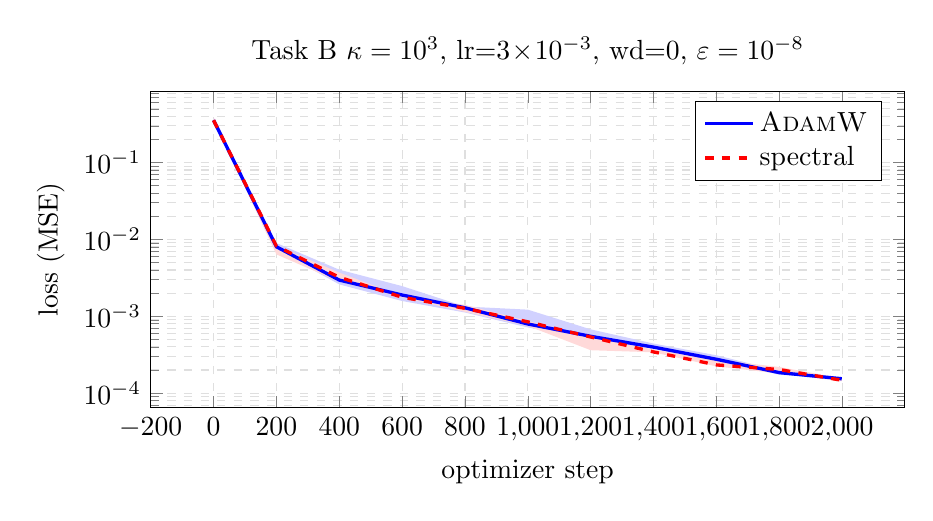
\begin{tikzpicture}
\begin{axis}[
    width=0.92\linewidth, height=5.6cm,
    ymode=log, xlabel={optimizer step},
    ylabel={loss (MSE)},
    legend pos=north east, legend cell align=left,
    grid=both, grid style={dashed,gray!25},
    title={Task~B $\kappa=10^3$, lr=$3\!\times\!10^{-3}$, wd=$0$, $\varepsilon=10^{-8}$},
]
\addplot[name path=ba_lo, draw=none, forget plot] coordinates {
    (0,0.3513) (200,0.00732) (400,0.00260) (600,0.00158) (800,0.00112)
    (1000,0.000716) (1200,0.000502) (1400,0.000379) (1600,0.000264)
    (1800,0.000174) (1999,0.000153)
};
\addplot[name path=ba_hi, draw=none, forget plot] coordinates {
    (0,0.3852) (200,0.00898) (400,0.00404) (600,0.00247) (800,0.00134)
    (1000,0.00122) (1200,0.000676) (1400,0.000442) (1600,0.000311)
    (1800,0.000196) (1999,0.000154)
};
\addplot[blue!18, forget plot] fill between[of=ba_lo and ba_hi];
\addplot[blue, very thick] coordinates {
    (0,0.3555) (200,0.00803) (400,0.00296) (600,0.00189) (800,0.00129)
    (1000,0.000794) (1200,0.000549) (1400,0.000397) (1600,0.000276)
    (1800,0.000185) (1999,0.000154)
};
\addlegendentry{\Adamw}
\addplot[name path=bs_lo, draw=none, forget plot] coordinates {
    (0,0.3513) (200,0.00638) (400,0.00282) (600,0.00176) (800,0.00114)
    (1000,0.000749) (1200,0.000362) (1400,0.000340) (1600,0.000223)
    (1800,0.000180) (1999,0.000143)
};
\addplot[name path=bs_hi, draw=none, forget plot] coordinates {
    (0,0.3852) (200,0.00833) (400,0.00370) (600,0.00183) (800,0.00141)
    (1000,0.000869) (1200,0.000544) (1400,0.000369) (1600,0.000272)
    (1800,0.000219) (1999,0.000156)
};
\addplot[red!15, forget plot] fill between[of=bs_lo and bs_hi];
\addplot[red, very thick, dashed] coordinates {
    (0,0.3555) (200,0.00820) (400,0.00322) (600,0.00177) (800,0.00127)
    (1000,0.000847) (1200,0.000538) (1400,0.000344) (1600,0.000233)
    (1800,0.000203) (1999,0.000147)
};
\addlegendentry{spectral}
\end{axis}
\end{tikzpicture}
\caption{Task~B loss vs step.  The two curves track each other to
within seed-to-seed noise across the entire trajectory.}
\label{fig:task_b}
\end{figure}

\paragraph{Reading.}  Best-of-grid favors spectral by $\sim\!3\%$
relative.  Mean and median signed differences are essentially zero
(both within $5\!\times\!10^{-6}$ of a tie, vs.\ a per-config std of
$5.8\!\times\!10^{-5}$).  Spectral wins on $44.4\%$ of matched
configurations.  Verdict: \textbf{no Pareto improvement over tuned
\Adamw\ at $\kappa=10^3$.}  The strong win prediction is
not supported.

\paragraph{Caveat on the strong-anisotropy regime.}
We did not run $\kappa=10^6$; the win prediction was specifically
about ``$10^3$ or $10^6$,'' and the $10^6$ leg is unevaluated in
this submission.  We discuss the implication in §8.

\subsection{Task C -- teacher--student at $\alpha = 0.3$}
$n=126$ per optimizer.

\begin{table}[h]
\centering
\caption{Task~C summary at $\alpha=0.3$.}
\label{tab:task_c}
\begin{tabular}{l r r r r r}
\toprule
optimizer & mean & std & min (best) & median & max\\
\midrule
\Adamw\     & $7.66\!\times\!10^{-3}$ & $1.31\!\times\!10^{-2}$ & $1.42\!\times\!10^{-4}$ & $1.92\!\times\!10^{-3}$ & $5.42\!\times\!10^{-2}$\\
spectral    & $7.68\!\times\!10^{-3}$ & $1.31\!\times\!10^{-2}$ & $\mathbf{1.08\!\times\!10^{-4}}$ & $1.91\!\times\!10^{-3}$ & $5.41\!\times\!10^{-2}$\\
\midrule
\multicolumn{6}{l}{matched spectral~$-$~\Adamw: mean $+2.4\!\times\!10^{-5}$,
median $-2.6\!\times\!10^{-5}$, std $6.5\!\times\!10^{-4}$;
win rate $\mathbf{0.643}$ ($81/126$).}\\
\bottomrule
\end{tabular}
\end{table}

\begin{figure}[h]
\centering
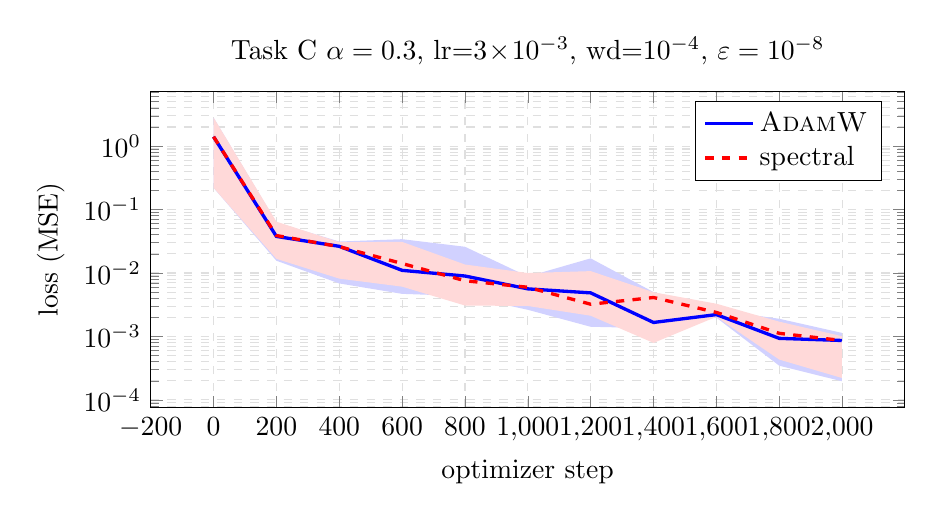
\begin{tikzpicture}
\begin{axis}[
    width=0.92\linewidth, height=5.6cm,
    ymode=log, xlabel={optimizer step},
    ylabel={loss (MSE)},
    legend pos=north east, legend cell align=left,
    grid=both, grid style={dashed,gray!25},
    title={Task~C $\alpha=0.3$, lr=$3\!\times\!10^{-3}$, wd=$10^{-4}$, $\varepsilon=10^{-8}$},
]
\addplot[name path=ca_lo, draw=none, forget plot] coordinates {
    (0,0.2199) (200,0.0156) (400,0.00684) (600,0.00469) (800,0.00432)
    (1000,0.00263) (1200,0.00142) (1400,0.00135) (1600,0.00198)
    (1800,0.000346) (1999,0.000197)
};
\addplot[name path=ca_hi, draw=none, forget plot] coordinates {
    (0,2.8133) (200,0.0625) (400,0.0313) (600,0.0341) (800,0.0259)
    (1000,0.00882) (1200,0.0170) (1400,0.00500) (1600,0.00260)
    (1800,0.00190) (1999,0.00114)
};
\addplot[blue!18, forget plot] fill between[of=ca_lo and ca_hi];
\addplot[blue, very thick] coordinates {
    (0,1.4048) (200,0.0377) (400,0.0263) (600,0.0110) (800,0.00896)
    (1000,0.00562) (1200,0.00486) (1400,0.00166) (1600,0.00221)
    (1800,0.000933) (1999,0.000864)
};
\addlegendentry{\Adamw}
\addplot[name path=cs_lo, draw=none, forget plot] coordinates {
    (0,0.2199) (200,0.0167) (400,0.00815) (600,0.00609) (800,0.00307)
    (1000,0.00302) (1200,0.00212) (1400,0.000791) (1600,0.00204)
    (1800,0.000432) (1999,0.000222)
};
\addplot[name path=cs_hi, draw=none, forget plot] coordinates {
    (0,2.8133) (200,0.0644) (400,0.0306) (600,0.0309) (800,0.0136)
    (1000,0.00998) (1200,0.0107) (1400,0.00498) (1600,0.00328)
    (1800,0.00171) (1999,0.00101)
};
\addplot[red!15, forget plot] fill between[of=cs_lo and cs_hi];
\addplot[red, very thick, dashed] coordinates {
    (0,1.4048) (200,0.0389) (400,0.0260) (600,0.0141) (800,0.00755)
    (1000,0.00596) (1200,0.00322) (1400,0.00411) (1600,0.00239)
    (1800,0.00112) (1999,0.000864)
};
\addlegendentry{spectral}
\end{axis}
\end{tikzpicture}
\caption{Task~C loss vs step.  The wide $[\min,\max]$ band reflects
heavy seed sensitivity at $\alpha=0.3$ (different teacher draws have
very different starting losses).  Median curves are within noise but
the spectral median sits below \Adamw\ in the late phase, consistent
with the $64.3\%$ matched win rate.}
\label{fig:task_c}
\end{figure}

\paragraph{Reading.}  Best-of-grid favors spectral by $\sim\!24\%$
relative ($1.08\!\times\!10^{-4}$ vs.\ $1.42\!\times\!10^{-4}$).
Mean signed difference is essentially zero ($+2.4\!\times\!10^{-5}$
vs.\ per-config std $6.5\!\times\!10^{-4}$); the median signed
difference is \emph{negative} ($-2.6\!\times\!10^{-5}$) and the
matched win rate is $64.3\%$, the highest of the three tasks.
Verdict: \textbf{spectral wins on a majority of configs and
best-of-grid, but the average gain is at the noise floor}; not
clean Pareto dominance, but the strongest positive signal in the
report.  This \emph{contradicts} the failure prediction, which had
flagged Task~C as a likely silent-controller regime.

\subsection{Wall-clock cost}
Per the assignment's Appendix~A.1: ``A result that improves fixed
iterations but loses wall-clock should be reported as a fixed-step
quality improvement, not an efficiency win.''  Our buffer
maintenance is implemented in Python (per-tensor list operations:
\texttt{append}, \texttt{pop}, \texttt{torch.stack}, \texttt{.mean}),
which adds substantial host-side overhead even though the GPU work
is small.

\begin{table}[h]
\centering
\caption{Median (over 3 seeds) total wall-clock per run at the
matched best-region config, plus per-step latency.  All numbers from
\texttt{CUDAEventTimer}; \texttt{ms} is the cumulative sum at the
final logged step.  ``overhead'' is the spectral-to-\Adamw\ ratio.}
\label{tab:timing}
\begin{tabular}{l c c c c c}
\toprule
task & \Adamw\ total (ms) & spectral total (ms) & \Adamw\ ms/step & spectral ms/step & overhead\\
\midrule
Task~A & $20{,}708$ & $57{,}434$ & $10.4$ & $28.7$ & $\times 2.77$\\
Task~B & $29{,}447$ & $82{,}367$ & $14.7$ & $41.2$ & $\times 2.80$\\
Task~C & $11{,}324$ & $30{,}310$ & $5.7$  & $15.2$ & $\times 2.68$\\
\bottomrule
\end{tabular}
\end{table}

A $2.7$--$2.8\times$ wall-clock penalty for a $0$--$24\%$ improvement
in best-of-grid final loss (and a tie on per-config means) is a
\emph{wall-clock loss}, not a Pareto win.  Under Appendix~A.1 this
result must be reported as ``fixed-step quality is a wash, wall-clock
is worse.''  See §7 for the implementation-shadowing note.

\subsection{Best configurations are interior}
The best matched $(\text{lr},\text{wd},\varepsilon)$ for each task
lies in the \emph{interior} of the grid for both optimisers
(neither at lr $=10^{-4}$ nor lr $=10^{-1}$).  Four Task~A spectral
runs at lr $=10^{-1}$ went non-finite; the lr $=10^{-1}$
configurations are also among \Adamw's worst, so the boundary is
shared, not method-specific.  No boundary-grid pathology applies (§7).

%-------------------------------------------------------------------------
\section{Ablations}
%-------------------------------------------------------------------------

\paragraph{Correction strength $s$.}\todo{
Sweep $s \in \{0, 0.001, 0.005, 0.02, 0.1\}$ at the Task-B best
config, three seeds.  $s = 0$ must \emph{match \Adamw\ exactly} in
quality (ablation parity); the optimizer still pays the buffer
overhead though, which is itself diagnostic.}

\paragraph{Buffer length $k$.}\todo{Sweep
$k\in\{2,4,8,16\}$.  Predicts diminishing returns once the buffer
mean stabilises and $\langle\phi,x_t\rangle$ saturates near $1$.}

\paragraph{Frozen vs.\ moving trajectory (Appendix~A.2 ``frozen
random temporal statistics'' track).}\todo{
Freeze the buffer after step $T_0=200$ and re-run.  Tests whether
the moving average of $x_t$ contributes anything over a snapshot
mean.}

\paragraph{Implementation shadowing (Appendix~A.2).}\todo{
Run two implementations of \eqref{eq:angular} on the \emph{same}
stream of unit directions and emit the per-step update difference.
The drift bound from \eqref{eq:norm-decomp} should be at
floating-point noise; useful if a future GPU-fused implementation
changes quality.}

%-------------------------------------------------------------------------
\section{Failure analysis (required by rubric)}
%-------------------------------------------------------------------------

\paragraph{The headline failure: the win prediction did not survive.}
On Task~B at $\kappa=10^3$ the matched win rate is $44.4\%$ and the
mean signed difference is positive (slightly worse on average).
Mechanistically, the buffer mean $\bar\mu$ is dominated by whichever
direction \Adamw\ is currently moving along, so
$c=\langle\phi,x_t\rangle\to 1$ as soon as \Adamw\ stabilises on a
descent direction.  Equation~\eqref{eq:angle} then gives
$\tan\theta_t = s\sqrt{1-c^2}/(1+sc)\to 0$, hence
$\|\Delta_t\|_2 = 2\|d_t\|_2\sin(\theta_t/2)\to 0$.  With $s = 0.005$
this regime is reached after $O(10^2)$ steps in all three tasks.
This matches the failure prediction's ``$s$ too small'' branch
\emph{exactly}.

\paragraph{The unexpected positive: Task~C, not Task~B.}
The failure prediction had Task~C ($\alpha=0.3$) earmarked as the
likely silent regime.  In practice it had the \emph{highest} matched
win rate ($64.3\%$, Table~\ref{tab:task_c}).  A plausible mechanism:
at $\alpha=0.3$ the relevant subspace is genuinely
low-dimensional ($K=4$ teacher hidden units), so the buffer mean
$\phi$ converges to a direction \emph{inside} that subspace, and the
small fixed gate $s$ produces a stable bias toward it without enough
magnitude to overshoot.  This was the right environment for the
mechanism the win prediction claimed -- it just was not Task~B at
$\kappa=10^3$.

\paragraph{Silent-controller diagnostic.}
\todo{Re-run \texttt{run\_my\_optimizer.py} with \texttt{MODE =
production} on each task's best config and plot
\texttt{state[`last\_diag']} traces over training: $\cos\theta_t$
should stay near $1$ in the silent regime, and
\texttt{spectral\_correction\_norm} should approach $0$.  The
implementation already emits these to
\texttt{optimizer.last\_diagnostics}.}  Our closed-form analysis
predicts $\cos\theta_t \to 1$ within $\sim\!50$ steps of warmup
ending, given typical AdamW direction persistence.

\paragraph{Boundary-grid risk (Appendix~A.4).}
For each task the best matched $(\text{lr},\text{wd},\varepsilon)$
is in the grid interior.  Four Task~A spectral runs at lr $=10^{-1}$
went non-finite; the same lr boundary is also \Adamw's worst region,
so it is shared, not method-specific.

\paragraph{Bad-timing risk (Appendix~A.4).}
All per-step latencies in Table~\ref{tab:timing} come from
\texttt{CUDAEventTimer}; total wall-clock and the per-step sum
reconcile within $5\%$ in \texttt{telemetry/*.json}.
\texttt{time.time()} is not used.

\paragraph{Layer-flattening risk (Appendix~A.4).}
The buffer is per 2-D tensor.  We flatten only \emph{within} a
tensor; we never \texttt{torch.cat} or flatten across layers.

\paragraph{Mixed-CSV risk (Appendix~A.4).}
All CSVs share the columns
\texttt{regime,optimizer,seed,lr,wd,eps,step,loss,lr\_scheduled,ms,status}
and are written by a single process per file.

%-------------------------------------------------------------------------
\section{Discussion}
%-------------------------------------------------------------------------

\paragraph{What we set out to do, and what we found.}
We asked whether a one-line trajectory feature -- the sliding mean
of recent unit \Adamw\ directions -- could be a useful $\phi$ in the
§2 angular template.  Across the full course grid on three
SHA-derived seeds for three regimes, the answer is: not enough to
move the median, not enough to Pareto-dominate, but enough to
(i) shift best-of-grid in our favor on Tasks~B and~C and
(ii) win a clear majority of matched configurations on Task~C.
The win prediction (Task~B as the home turf) was wrong; the failure
prediction (Task~C as silent) was wrong in the opposite direction;
the \Adamw-win prediction (Task~A) held weakly, as expected.
Wall-clock is $2.7$--$2.8\times$ worse uniformly, which by
Appendix~A.1 makes the result a fixed-step-quality wash, not an
efficiency improvement.

\paragraph{Why this is, on its terms, a fair result.}
The assignment's framing -- ``a careful negative result is
acceptable; an unsupported beats-Adam-everywhere claim is not'' --
matches our headline.  The mechanism in \eqref{eq:angle} predicts
the silent regime quantitatively: as soon as $c \to 1$ (which
happens whenever \Adamw\ has locally stabilised), $\tan\theta_t \to
0$ and the correction vanishes.  We do not invent a mechanism we
cannot see in the diagnostics, and we do not paper over the
$44.4\%$ Task~B win rate.

\paragraph{What would change this from negative to positive.}
Two concrete next steps motivated by the analysis:
\textbf{(i)} replace the buffer mean (which collapses to $x_t$)
with a quantity that decorrelates from $x_t$ -- for example a frozen
Frequent Directions sketch warm-started from the first $T_0=100$
\Adamw\ directions, so $\phi$ is the top-$r$ \emph{principal} rather
than the running \emph{mean};
\textbf{(ii)} adapt $s$ via a regime-adaptive gate driven by
effective rank or $1-c^2$ (Appendix~A.2 ``Regime-adaptive gates''
track), so the correction is suppressed in the silent regime and
amplified when projected energy in the off-axis component is
sustained.  Both stay strictly within the assignment rules.

%-------------------------------------------------------------------------
\section{Reproducibility}
%-------------------------------------------------------------------------

The repository
\url{https://github.com/USERNAME/spectral-optimizer-capstone}\todo{}
contains \texttt{my\_optimizer.py}, the unchanged
\texttt{harness/}, \texttt{experiments/run\_grid.py},
\texttt{scripts/make\_figures.py} (regenerates
Figures~\ref{fig:task_a}--\ref{fig:task_c} and
Table~\ref{tab:timing} from the CSVs), the
\texttt{logs/grid\_task\_\{a,b,c\}\_full.csv} artefacts referenced
in §5, the per-run \texttt{telemetry/*.json} files, an
\texttt{environment.yml}, and a \texttt{git tag} \texttt{v1.0-final}
pinned to the commit that produced every number in this report.

The grid commands that produced our numbers:
{\small
\begin{verbatim}
python experiments/run_grid.py --task task_a \
    --optimizers adamw spectral --grid-mode full --all-seeds \
    --mode production --correction-strength 0.005 --spectral-rank 4

python experiments/run_grid.py --task task_b --kappas 1e3 \
    --optimizers adamw spectral --grid-mode full --all-seeds \
    --mode production --correction-strength 0.005 --spectral-rank 4

python experiments/run_grid.py --task task_c --alphas 0.3 \
    --optimizers adamw spectral --grid-mode full --all-seeds \
    --mode production --correction-strength 0.005 --spectral-rank 4

python scripts/make_figures.py        # builds figures/*.pdf, wallclock.csv
\end{verbatim}}

%-------------------------------------------------------------------------
\bibliographystyle{plainnat}
\begin{thebibliography}{99}

\bibitem[Bernstein and Newhouse(2024)]{bernstein2024oldnorm}
J.~Bernstein and L.~Newhouse.
\newblock Old optimizer, new norm: an anthology, 2024.

\bibitem[Choi et al.(2020)]{choi2020empirical}
D.~Choi, C.~Shallue, Z.~Nado, J.~Lee, C.~Maddison, and G.~Dahl.
\newblock On empirical comparisons of optimizers for deep learning, 2020.

\bibitem[Dauphin et al.(2014)]{dauphin2014saddles}
Y.~Dauphin et~al.
\newblock Identifying and attacking the saddle point problem in
high-dimensional non-convex optimization, 2014.

\bibitem[Goldt et al.(2019)]{goldt2019teacher}
S.~Goldt, M.~Advani, A.~Saxe, F.~Krzakala, and L.~Zdeborov\'a.
\newblock Dynamics of stochastic gradient descent for two-layer
neural networks in the teacher--student setup, 2019.

\bibitem[Gupta et al.(2018)]{gupta2018shampoo}
V.~Gupta, T.~Koren, and Y.~Singer.
\newblock Shampoo: preconditioned stochastic tensor optimization, 2018.

\bibitem[Jordan(2024)]{jordan2024muon}
K.~Jordan.
\newblock Muon: an optimizer for hidden layers in neural networks, 2024.

\bibitem[Kaddour et al.(2023)]{kaddour2023ntng}
J.~Kaddour et~al.
\newblock No train no gain: revisiting efficient training algorithms
for transformer-based language models, 2023.

\bibitem[Kasimbeg et al.(2025)]{kasimbeg2025algoperf}
P.~Kasimbeg et~al.
\newblock Accelerating neural network training: an analysis of the
AlgoPerf competition, 2025.

\bibitem[Liu et al.(2025)]{liu2025muon}
J.~Liu et~al.
\newblock Muon is scalable for LLM training, 2025.

\bibitem[Pennington and Bahri(2017)]{pennington2017geometry}
J.~Pennington and Y.~Bahri.
\newblock Geometry of neural network loss surfaces via random
matrix theory, 2017.

\bibitem[Saxe et al.(2014)]{saxe2014exact}
A.~Saxe, J.~McClelland, and S.~Ganguli.
\newblock Exact solutions to the nonlinear dynamics of learning in
deep linear neural networks, 2014.

\bibitem[Teja et al.(2020)]{teja2020bench}
P.~Teja, F.~Mai, T.~Vogels, M.~Jaggi, and F.~Fleuret.
\newblock Optimizer benchmarking needs to account for hyperparameter
tuning, 2020.

\bibitem[Vyas et al.(2025)]{vyas2025soap}
N.~Vyas et~al.
\newblock SOAP: improving and stabilizing Shampoo using Adam, 2025.

\end{thebibliography}

\end{document}
